\begin{center}
\textbf{Курсовая работа}\\
\end{center}
~\\
\textbf{\textit{Тема:}}
Расчет параметров двигателя на квазистационарных режимах\\
~\\
\textbf{\textit{Цель работы:}}
В данной работе выполняется расчет на ПЭВМ параметров рабочих процессов двигателя с заданной начальной формой заряда. По результатам расчетов определяется изменение во площади поверхности горения, давление в камере сгорания, параметры потока по длине сопла и изменение тяги двигателя во время работы РДТТ.
\begin{center}
\textbf{\textit{Общие положения и теоретические сведения}}

\end{center}
На стационарном режиме работы РДТТ в каждый момент времени устанавливается баланс между приходом продуктов сгорания от твердого топлива и расходом продуктов сгорания через сопло. Учитывая, что поверхность горения заряда ТТ (в общем случае) не остается величиной постоянной, то баланс массы для продуктов сгорания в газовом объеме КС должен описываться дифференциальным уравнением вида
\begin{equation}\label{eq:fourierrow} 
\frac{dm}{dt}= \frac{d(\rho V_k)}{dt} = P_T - G_c
\end{equation}\\
где масса продуктов сгорания в КС, плотность продуктов сгорания, свободный объем камеры сгорания, секундный массовый приход продуктов приходом продуктов сгорания от твердого топлива, расход продуктов через выходное сопло.\\
При запуске двигателя давление в камере сгорания постепенно нарастает до тех пор, пока не достигнет некоторого заданного уровня, что эквивалентно накоплению массы газа и энергии в газовой зоне камеры сгорания. Приход продуктов при запуске двигателя превышает расход продуктов сгорания через сопло и этому, в частности, способствует дополнительный приход продуктов сгорания при работе воспламенителя.\\
При выходе на стационарный режим приход и расход продуктов уравновешивают друг друга. Приход и расход продуктов сгорания будет в процессе работы двигателя изменяться в определенных пределах, на характерные времена установления режима в КС часто гораздо меньше характерных времен изменения параметров рабочего процесса. Это относится к основным режимам работы (стационарным или квазистационарным) и должно быть получено соотношение, позволяющее найти параметры для расчета стационарные режимы энергосистем.\\
~\\
Приход продуктов в камере сгорания определяется массой сгоревшего топлива за единицу времени: \\
\begin{equation}\label{eq:fourierrow} 
P_t = V_g * \rho_T 
\end{equation}\\


\begin{flushright}
\begin{scriptsize}
\textit{160700.65   Проектирование авиационных и ракетных двигателей\\
 Информационные технологии в АКТ: Лабораторный практикум} \\
\end{scriptsize}
\end{flushright}
\begin{equation}\label{eq:fourierrow} 
V_g = S_g * u 
\end{equation}
\begin{equation}\label{eq:fourierrow} 
P_t = \rho_T * S_g * u,
\end{equation}
где объем сгоревшего топлива в единицу времени, плотность топлива, скорость горения ТТ.\\
~\\
Скорость химических реакций существенно зависит от давления. Из-за сложного механизма взаимодействия газовой и конденсированной зон, конкурирующих процессов тепло-массопереноса для описания процесса горения твердого топлива часто используют эмпирические законы для скорости горения. В частности, для зависимости скорости горения топлива от давления может быть использован степенной закон для скорости горения:\\
\begin{equation}\label{eq:fourierrow} 
u = u_1 * {(\frac{P_k}{P_1})}^v = u(P_k)
\end{equation}\\
где p1 – некоторый выбранный уровень давления, который является характерным для работы топлива данного типа.\\
В качестве уровня давления могут быть выбраны и стандартные условия для атмосферы, хотя при этих условиях топлива могут не гореть, и выполнятся просто перерасчет имеющихся данных о скорости горения к стандартным условиям. \\
\begin{equation}\label{eq:fourierrow} 
u = u_{10} * {(\frac{P_k}{P_0})}^v = u_1 * {(\frac{P_k}{P_1})}^v
\end{equation}\\
\begin{equation}\label{eq:fourierrow} 
u_{10} = u_1 * {(\frac{P_0}{P_1})}^v
\end{equation}\\
Часто используют приведенные скорости горения к стандартным условиям, но при этом оговаривают диапазон применения соотношений по давлению. Уравнение прихода газа запишем \\
\begin{equation}\label{eq:fourierrow} 
P_T = \rho * S_g *u_1 * {(\frac{P_k}{P_0})}^v
\end{equation}\\
Учитывая, что выходное сопло РДТТ после выхода двигателя на режим работает в режиме критическом или сверхкритическом режиме истечения, то расход продуктов через сопло определяется соотношением: \\
\begin{equation}\label{eq:fourierrow} 
G_{nozzle} = \frac{P_k F_{kr}}{\beta}
\end{equation}\\
где $\beta$ - расходный комплекс (имеет размерность скорости и для топлив принимает значение порядка 1400 – 1800 м/с).


\begin{flushright}
\begin{scriptsize}
\textit{160700.65   Проектирование авиационных и ракетных двигателей\\
 Информационные технологии в АКТ: Лабораторный практикум} \\
 \end{scriptsize}
\end{flushright}
Учитывая, что выполняется баланс между приходом и расходом продуктов, получил
\begin{equation}\label{eq:fourierrow} 
\rho_T * S_g * u_1 * {(\frac{P_k}{P_0})}^v = \frac{P_k * F_{kr}}{\beta}
\end{equation}\\
Из этого уравнения можем найти соотношение для расчета давления в камере сгорания pк, которое позволит по конструктивным параметрам энергосистемы и свойствам топлива найти параметры рабочего процесса на стационарных режимах.\\
Коэффициент в степенном законе горения может изменятся в диапазоне от 0 до 1. Большие значения $\nu$ соответствуют специальным топливам, используемых для в РДТТ с глубоким регулирования двигателя по тяге. Для обычных топлив $\nu$ принимает значения порядка 0,2…0,5.
Выполняем необходимые преобразования в уравнении баланса расхода
\begin{equation}\label{eq:fourierrow} 
P_k^\nu * \frac{\rho_T * S_g * u_1}{P_0^\nu } = \frac{P_k * F_{kr}}{\beta}
\end{equation}\\
\begin{equation}\label{eq:fourierrow} 
P_k^{\nu-1} * \frac{\rho_T * S_g * u_1 * \beta}{F_{kr} * P_0^\nu }
\end{equation}\
и получаем формулу Бори
\begin{equation}\label{eq:fourierrow} 
P_k = {(\frac{\rho_T * S_g * u_1 * \beta}{F_{kr} * P_0^\nu})}^{\frac{1}{1 - \nu}}
\end{equation}\\
Данное соотношение используется для определения основных параметров двигателя на расчетных режимах, для анализа возможностей регулирования двигателя, анализа возможных изменений параметров при нештатных режимах работы, оценок изменения параметров рабочих процессов в зависимости от технологических разбросов, по мере разгара критического сечения сопла и т.д..\\
\begin{center}
\textbf{\textit{Данные варианта:}}\\
~\\
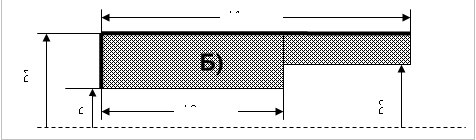
\includegraphics[width=7.4cm]{1} \\
\end{center}
\begin{flushright}
{\textit{Рис. №1: Форма заряда по варианту}}\\
\end{flushright}
\begin{center}
\begin{tabular}{  | c | c | c | c | }
\hline
N1 & N2 & N3 & N4 \\
\hline
Б & Б & В & A \\
\hline
\end{tabular}
\end{center}
~\\
\begin{flushright}
\begin{scriptsize}
\textit{160700.65   Проектирование авиационных и ракетных двигателей\\
 Информационные технологии в АКТ: Лабораторный практикум} \\
\end{scriptsize}
\end{flushright}
\begin{center}
\textbf{\textit{Исходные данные}}\\
\end{center}
\begin{flushright}
\textit{Таблица №2: Исходные данные}\\
\end{flushright}
~\\
